% +---------------------------------------------------------------+
% | Author :    Noémie Plancherel, HEIG-VD
% | Date :      April 1st, 2022
% +---------------------------------------------------------------+


\chapter{Planning}
Le travail de bachelor sera séparé en plusieurs tâches et sous-tâches différentes qui permettront de répartir plus facilement le travail sur des périodes de plusieurs semaines. Ci-dessous, le planning détaillé avec toutes les tâches : 

\begin{enumerate}
	\item Préparation
	\begin{itemize}
		\item Rédaction du cahier des charges
		\item Planification
		\item Recherches initiales et introduction
	\end{itemize}
	\item Étude de marché
		\begin{itemize}
			\item Recherches et explication des différents types de gestionnaires de mots de passe
			\item Comparaison des fonctionnalités
		\end{itemize}
	\item Étude sécuritaire
		\begin{itemize}
			\item Identification et analyse des menaces potentielles
			\item Rédaction des exigences sécuritaires
		\end{itemize}
	\item Sélection
		\begin{itemize}
			\item Mise en place des critères de sélection des candidats
			\item Sélection des candidats
		\end{itemize}
	\item Analyse sécuritaire (pour chaque candidat)
		\begin{itemize}
			\item Identification et rédaction des critères d'analyse 
			\item Analyse sécuritaire de chaque aspect
		\end{itemize}
	\item Synthèse (pour chaque candidat)
		\begin{itemize}
			\item Synthèse des résultats
			\item Rapport des faiblesses au fabricant
		\end{itemize}
	\item Synthèse générale
		\begin{itemize}
			\item Comparaison de tous les résultats
			\item Conclusion du travail
		\end{itemize}
	\item Documentation
		\begin{itemize}
			\item Rédaction du rapport
			\item Lecture / visualisation de documents
			\item Tenue d'un journal de travail
		\end{itemize}
\end{enumerate}

Un diagramme de Gantt a également été effectué afin de pouvoir visualiser le planning et ajouter des périodes de temps :
\begin{center}
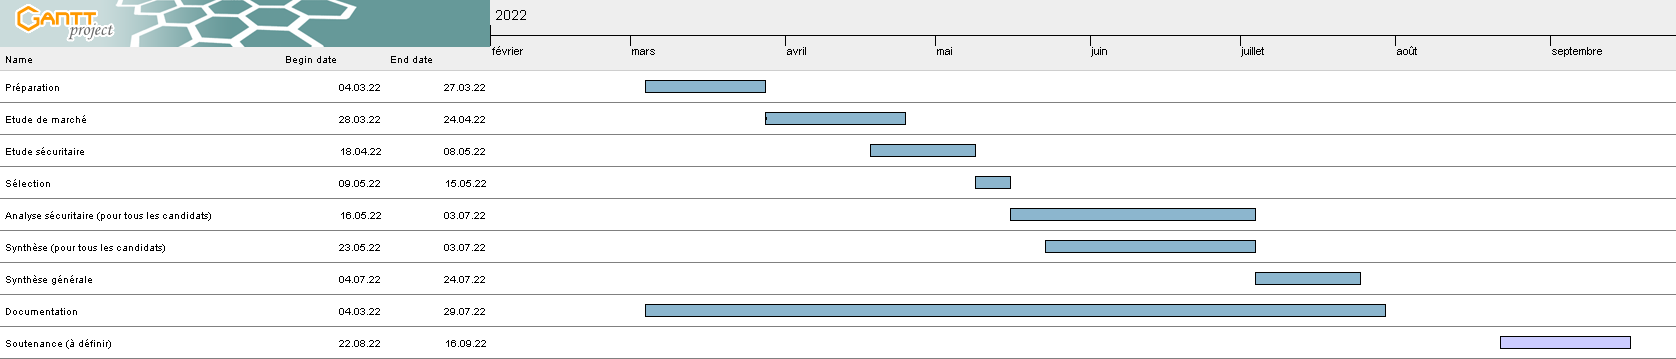
\includegraphics[width=15.5cm]{images/planning.png}
\end{center}
